\documentclass[conference]{IEEEtran}
\usepackage[utf8]{inputenc}
\usepackage[pdftex]{graphicx}
\usepackage[utf8]{inputenc}
\usepackage[T1]{fontenc}
\usepackage{graphicx}
\usepackage[space]{grffile}
\usepackage{longtable}
\usepackage{float}
\usepackage{wrapfig}
\usepackage{amssymb}
\usepackage{hyperref}
\usepackage{caption}
\usepackage{epstopdf}
\usepackage[pdf]{pstricks}
\usepackage{subcaption}
\usepackage{cite}
%\usepackage{subfigure}
\DeclareGraphicsExtensions{.eps}
%opening
\title{Large Scale Web Page Optimization of Virtual Labs}
\author{Jatin Agarwal, Utkarsh Rastogi, Prateek Pandey, Maddala Saraswati Soumya and Venkatesh Chopella}

\begin{document}

\maketitle

\begin{abstract}
We propose web page optimization as necessary step in web application
development. In context of virtual labs, several online experiments were designed by domain
experts from various disciplines and thousands of web pages were developed.
But domain expert did not know best practices for web development, therefore
webpages had lot of performance issues on client side. So end user suffered slow
rendering of pages on the client side.
Performance of an web application largely depends upon the content of the web
page because rendering takes place on client side. 
And client machine may have limited resources at his side. Therefore web page
optimization seems necessary step to improve user experience.
In contrast to existing work on this field, here we focus on large scale web
performance analysis through data visualization. Based on this large scale visualization,
we present a utility of existing web optimization tool by experimentation on a
MHRD web project ``virtual labs''.
\end{abstract}

\section{Introduction}\label{sec-2}
After onset of world wide web, performance of web implied optimizing the server side but nowadays
optimization on the client side has become bottle neck because of complex web
application. Now days, front-end developers use a lot of critical resources like
javascipt, CSS and images to make a good user interface which becomes
overhead during page rendering which means lesser user experience. Success of a web
application is judged based on user's experience which also includes fast response
time. Optimized web pages not only render a web page fast but also saves network
bandwidth. Along with a good responsive web page, web developers should
also focus on optimizing critical resources by minifying size and number of resources
Critical rendering path is the chain of necessary events that
occurs to render webpage on browser. The main critical resources on a web
pages are CSS, javascript and images. For each critical resource on a
webpage, browser makes a new request to server. CSS and javascript are the two
critical resources that blocks the rendering of a webpage. Therefore, correct
sequence of http requests can reduce the perceived page load time which means page
load time will not reduce in reality but critical resources needed to render webpage are
fetched first and remaining resources are fetched in background. Therefore,
while optimizing web page for speed we should focus on 
\begin{enumerate}
 \item Minifying size of critical resources
 \item Minifying number of critical resources
 \item Minifying critical rendering path.
\end{enumerate}

The goals of our experimentation, performed in collaboration with VLEAD,
IIIT-Hyderabad were :

\begin{itemize}
\item To analyze performance of thousands of web pages hosted at virtual labs.
\item To evaluate the utility of the Pagespeed with respect to optimizing web pages of virtual labs.
\item Comparison between the web performance of virtual labs web pages with
and without a web optimization like Google PageSpeed tool inoder
\end{itemize}

\section{Background}\label{sec-3}
Initially when world wide web started most of the web pages where plain hyper text documents.
Slowly people started sharing media content like images and audio on web and in past decade
web pages got transformed into web application with depends upon on critical resources
like CSS, javascript and media content like images, audio, video etc. Now rendering of webpages depends upon
following three major criteria`s. Firstly order in which critical resources are fetched, secondly on
number of critical sources and lastly on size of critical resources. Web gaints like Yahoo and Google
have listed best practices for web developers to improve performance of web pages. So now we briefly
explain some of the best practices in order to appreciate significance of web performance optimization.
\begin{itemize}
\item \textbf{Minimize http requests :}
Number of http requests to render any web page is directly proportional to
number of critical resources.
For each critical resource in the page, browser have to make a new http request 
to server and then its get loaded. So, almost 80\% of the response time is
consumed in downloading all the resources. So to reduce number of http
requests, one can combine multiple CSS into one, also multiple javascipt files can
be combined into one. Other ways include image spriting, etc.

\item \textbf{Use a Content Delievery Networks :}
The nearest geographical server is selected for delivering the content which reduces load time.

\item \textbf{Add Cache Control Header :}
For static components, setting far future expires header will reduce number of http request
so that browser can fetch resources from cache when request to same webpage is made again.
For dynamic components, use an appropriate Cache control header to help browser
with conditional requests. This reduces unnecessary http requests.

\item \textbf{Gzip components :}
Compression reduces response time by reducing the size of http response.
Gzip is most popular and effective compression method at this time. It reduces
response time by 70\%. If a web client indicates for support for compression in
the http request header, server sends a compressed components.

\item \textbf{Stylesheets at the Top: }
Problem with not including link to style sheets in the head tag is that it blocks
progressive rendering and till the style sheets are not fetched users sees nothing
on screen.

\item \textbf{Put Scripts at Bottom :}
Putting scripts at the top, blocks parallel downloading of resources from same host.
In most of the cases scripts are needed when users starts interacting with the web page. 

\item \textbf{Make Inline Small CSS and javascript files :}
If file size is to small, then it should be made inline as it will reduce number
of http requests.

\item \textbf{Make large css and javascript file external :}
CSS and javscript files are cached by browser. So we avoid downloading it every time a request is made.
First time it will take time to download but all later requests are served from the user's browser cache.

\item \textbf{ Minify javascript and css :}
Unnecessary characters from code should be reduced which includes removing
comments, redundant code and removing white spaces. Removing this unnecessary
characters reduces number of critical bytes served to client-side and increases response time.

\item \textbf{Avoid Redirects :}
Connecting an old page to new one takes leads to an extra cycle of dns lookup and tcp handshake adding latency
and delaying the response. Therfore, it should be avoided.

\item \textbf{Configure ETags :}
Entity tags is a way that browser and server use to determine whether the
component in cache is same as that on server.

\item \textbf{Flush the buffer early :}
It allows to send partially ready response to browser.It should be written as
early as possible in the code, preferably in the head section.
In php there is function flush() to flush the buffer. 

\item \textbf{No 404 error :}
Http requests made and getting a response like 404 Not found is totally useless
and it increases response time.

\item \textbf{Make favicon small and cacheable :}
Favicon stays in the core of server and  it is necessary because if its missing,
browser will still request for it and adding to the latency.
\end{itemize}

Yahoo {\bf Yslow} and {\bf Google Pagespeed} are well known tools that are capable of
evaluating webpages performance and providing suggestions to optimize webpages
based on the best practices listed above. But the pagespeed is more than a performance analysis
tool and is also capable of optimizing webpages without changing semantics of a webpage.

Yahoo yslow.js is javascript API which runs on phantomjs. PhantomJS is a
headless browser with JavaScript API. We used Yslow as performance measuring
tool because it not only analyzes a webpage but gives suggestions on how to
improve it.
It works on three process:
\begin{itemize}
\item It crawls the DOM to find each component.
\item Collects information for each component and analyzes each of them.
\item It generates scores out of 100 for each rule which produces the overall
score for page.
\end{itemize}
The grades for individual rules are computed differently depending on the rule.
For example, for Rule 1, three external scripts are allowed and each extra script
four points are deducted from the overall weight. The code for grading each
rule is found in rules.js. The overall grade is a weighted average of the
individual grades for each rule, calculated in controller.js The rules are
approximately in order of importance, most important first. The specific weights
are in the ruleset objects in rules.js. Score computation is shown in
the following table no 1 in Appendix section.

Mod\_pagespeed is an automated web page optimization tool developed by Google for
optimization of web pages. It not only
analyzes a web page but also optimizes it. Based on best practices, it has
certain set of filters which optimizes web page during run time. As the server
gets request for the webpage, it dynamically rewrites the page using its filters
and sends a highly optimized page. The rewriting happens only when the first
request for web page is made and for all later request web page is served from the cache
at server side. There are total of 40+ filters which supports
optimization. These filters can be turned on or off based on requirements. 
% \begin{center}
% \begin{tabular}{lll}
%  Rule                               &  Configs                     & Computation                 \\
%  Make fewer HTTP requests           &  N(JS-3)*3                   &            
%                  \\
%                                     &  max images=6                & 
% N(images-6)*3               \\
%                                     &  max css=2                   &  N(CSS-2)*4
%                  \\
%  Use a CDN                          &  patterns=CDN hostname       &  N RegExp
% mismatches*10      \\
%  Avoid empty src or href            &                              &  N empty
% tags*100            \\
%  Add Expires headers                &  how far=172800s             &  N(expiring
% 2 days)*11       \\
%  Compress components with GZip      &  min file size = 500 bytes   & 
% N(uncompressed file) * 11   \\
%  Put CSS at top                     &                              &  1+N link
% tag on BODY*10     \\
%  Put JavaScript at bottom           &                              &  N JS on
% HEAD * 5            \\
%  Reduce DNS lookups                 &  max domains = 4             &  (N domains
% - 4) * 5         \\
%  Minify JavaScript and CSS          &  types = js, css             & 
% N(unminified JS or CSS)*10  \\
%  Avoid URL redirects                &                              &  N
% redirects * 10            \\
%  Remove duplicate js and CSS        &  types = js, css             &  N
% (duplicated JS or CSS)*5  \\
%  Configure ETags                    &  types=js,css,image,flash    &  N bad etag
% of any type*11   \\
%  Reduce the number of DOM elements  &  range = 250,max dom = 900   &            
%                  \\
%  Avoid HTTP 404 (Not Found) error   &  types=js,css,image,favicon  &  N 404 * 5 
%                  \\
% \end{tabular}
% \end{center}
% 
% 
% 
% Grade Computation From Score
% 
% 
\begin{center}
\begin{tabular}{rl}
    Score  &  Grade  \\
   95-100  &  A+     \\
    90-94  &  A-     \\
    85-89  &  B+     \\
    80-84  &  B-     \\
    75-79  &  C+     \\
    70-74  &  C-     \\
    65-69  &  D+     \\
    60-64  &  D-     \\
    55-59  &  E+     \\
    50-54  &  E-     \\
 Below 50  &  F      \\
\end{tabular}
\end{center}

\section{Approach}\label{sec-4}
Our work is broadly divided into four major phases namely Data Collection, Data
Visualization, Analysis of Data and optimizing web pages based on analysis.
During data collection phase we first collected all the urls of virtual labs
hosted at IIIT-Hyderabad. Then we collected Yslow reports for each web page
using an automated script and phantomJS. After collecting all the reports we
extracted scores for each rule from reports and stored it in a csv file. During
visualization phase all data is visualized using an automated script indicating
performance for each rule and also overall performance of web pages. Later we
did analysis for optimized pages of virtuals labs.

\subsection{Urls and Report Collection}\label{sec-4.1}
As first step to collect data and generate reports, we
collected urls of all the webpages at following domain deploy.virtuals-labs.ac.in hosted at
IIIT-Hyderabed. Since we have access to server, to get all the urls, we wrote an
automated bash script to extract all the html and php pages links from the
server and stored it into the text file.
To test the performance of vlab.co.in, we also collected the 5000 urls for this
website. This time since we do not have the access of server ,we used an online
sitemap generator to get the urls.
We wrote an automated script to generate the reports for each web page using
yslow.js and phantomJS. This automated script read a url from a file containing
all the urls and generate report for each web page. In this script, we are making
ten phantomjs call as background process for ten different webpages. For urls which are inactive, failed reports will
be generated and we are pushing that url into the failed urls file and deleting
the failed reports. These reports serves as input to CSV file generation.

\subsection{CSV File Generation}\label{sec-4.2}
CSV file are generated using a bash script. This CSV file will contain the overall
score and scores corresponding to each rule. Script will extract all the scores
for corresponding rule and will dump into the CSV file line by line. The
content in the CSV file will be used for visualization.

\subsection{Visualization}\label{sec-4.3}
Visualization is done using python matplotlib and csvkit. We have written an automated
scripts to generate all the graphs needed for visualization. Scripts takes csv file as input
and set of bar graphs specific to each rule.

\section{Experimentation}\label{sec-5}

\subsection{www.vlab.co.in}\label{sec-5.1}
We started our experiment by collecting Yslow reports for vlabs. 
We collected 5000 urls of www.vlab.co.in. and generated
Yslow reports corresponding webpages and generated CSV file for the
scores. Finally, we plotted data accumulated in csv files and analyzed the
current status of webpages by looking at bar graphs.

\subsection{deploy.virtual-labs.ac.in without pagespeed}\label{sec-5.2}
This is the virtual lab website hosted at IIIT-Hyderabad. To analyze performance
of webpages, we collected all the urls located at deploy.virtual-labs.ac.in by using
our bash script. Total of 8786 urls were collected, reports were
generated for web page located at each url and scores were accumulated in csv file.
Later we visualized scores to analyze the current status of web pages.

\subsection{Optimization of deploy.virtual-labs.ac.in using mod\_pagespeed}\label{sec-5.3}
We made a replica of deploy.virtual-labs.ac.in server on a container. We installed
Google mod\_pagespeed on the container to see what extent pagespeed optimizes.
Then, we collected reports for all the web pages and
generated CSV file. After generating bar graphs we compared results with deploy.virtual-labs.ac.in without pagespeed
to observe how much optimization was done by pagespeed.

 \begin{figure}[ht]
  \centering
  $\includegraphics[scale=0.40]{img/vlab-co-in/Overall_Score.pdf}$
  \caption{Number of urls versus Overscore}
  \label{overallscore-vlab}
\end{figure}
\section{Analysis}\label{sec-6}
In this section we analyze web page performance of virtual-labs.ac.in in two different settings on data set containing 9000 web pages.
One when page speed module is installed on our system and other one without page speed. We also analyze web page performance of vlab.co.in  
on data set containing 5000 web pages.
\subsection{Analysis of vlabs.co.in}
 Out of 5000 urls we collected statistics for 4945 web pages.
\begin{itemize}
\item From the figure \ref{overallscore-vlab}, we can observe that only 1 web page is having good
performance. Rest of the web pages does not get good grades and need to be
optimized to improve performacne. Out of rest 687 i.e 13\% webpages are in above average conditions, 1038
webpages are performing average and rest 3220 webpages are not in good
condition. Therefore, statistics are shows that these pages are not following
performance best practices and performace of webpages can be improved.  
 
\item From the graph below, we can observe that all the webpages are having their
CSS files inside the head tag else they block the progressive rendering.

\item From the graph below, we can observe that all the webpages are having their
script files at the bottom else they block parallel downloading.

\item From the graph below, we can observe there is no usage of Content Delivery
Networks. Actually it should have been used for such large website so that page
rendering speed is high.

\item From the graph below, we can observe that there is no use of Expires
Headers in the wepages. This practice is not followed in the pages and it has to
fetch each static critical resources everytime page is requested as it is not
set expire far future.

\item From the graph below, we can observe that only 89 webpages out of 4945
pages are in compressed form and rest are in uncompressed form. This will lead to
large payload size and thus will increase network traffic and will slow page
rendering.
\item From the graph below, we can observe that this website does not use entity
tags. Due to this it has to download critical resources every time request for page is
made.
\item From the graph, we can see that all pages vlabs are having favicon for it.
\item from the graph, we can see that number of critical resources  on the pages
are more than required. Only 1 web page is getting A+ grade.Around 4500 webpages
have scores between 65 to 75 means they are loaded with multiple css, javascript
and images.For each resource, browser have to make a request to server and most
of the time is wasted downloading the resources.This resources  number should be
reduced for fast rendering.
\end{itemize}
\subsection{Optmization using Pagespeed.}\label{sec-6.2}

As we have generated statistics for 8986 webpages under
deploy.vitual-labs.ac.in and for replica of deploy server on which pagespeed has
been installed. Here we observed how much pagespeed optimizes the webpages.
\begin{itemize}
\item From the graphs, we can see that for deploy.virtual-labs.ac.in 4299 are in
A+ grades for \textbf{overall score} while with pagespeed this rises to 6051. It
shows pagespeed is imroving the performance of web pages by optimizing it. Also
we can see see without pagespeed only 1226 wepages are in A- grade but with
pagespeed it increased to 1667. From the graphs we can analyze that overall
performance of webpages has improved after using pagespeed.

\item From the graphs, we can observe that without pagespeed  mostly only 3214
webpages are in B+  and have \textbf{added expires headers} followed  and around
45\% are not follwing it. But with pagespeed, 4729 webpages were in B+ grade and
there was shift of number from low grades to high grades.

\item From the graphs, we can observe that most webpages are \textbf{compressed
using Gzip} and 8257 urls falls under A+ grades while with pagespeed this number
rises to 8761.

\item From the graphs,Please send your dress code request positively on or before 30th July, 2014.
we can see that w.r.t \textbf{Etags} without pagespeed
3535 pages have A+ grade, 831 have B+ grade, 384 have C+ grade, 3704 have score
less than 50 but with pagespeed this number shifted to more higher grades. We can
see now 6441 pages in A+ in comparison with 3534. But the major difference is seen
at below 50 score pages, now this have reduced to 633 in comparison to previous
3704.

\item From th graphs we can see that w.r.t \textbf{make fewer http
requests}, without pagespeed only 7791 webpages were in grade A+ and 461 pages
were in A- but with pagespeed 8202 pages were in A+ grades. Major shift was from 
A- grade to A+ grade. Rest pages shows no observable changes.

\item From the graphs, we can see that w.r.t \textbf{minified JavaScript and CSS}
without pagespeed 7059 webpages were in grade A+, 1395 pages in A-, then 254 in
B- and 20 were below F. After optimizing with pagespeed 8639 pages were in grade A+ ,94 in A- and only 3 below F.
\end{itemize}

\section{Conclusion}
\label{sec-7}
This paper is concerned about Web Page Optimization of virtual labs which means fast rendering and less
network bandwidth. This lead us to think us how to decrease the number and size of
resource and also how to decrease the perceived load time. These webpages consists
of critical resources like CSS, JavaScript and images. This optimization can be
achieved by minimizing the number of critical resources, minimizing the size of
critical resources and minimizing the critical path length.

 Our framework is helps in visualizing website performance and
it can be used to suggest lab developers to work on these best practices. Also it
gives the list of urls pages which are broken. Google Pagespeed is the automated web optimization
tool that comes as a saviour for optimizing webpages of already existing web applications. It has 40+
filters which optimizes page and can be used according to our requirement. Also,
it is open source and available for free. It should be used for huge websites like virtual labs
application developers comes various domains and backgrounds.
 
\section{Future Work}\label{sec-8}
This framework can be modified to give the list of urls of web pages that perform badly.
Generating report takes atleast 24 hrs to process 5000 urls but by
making phantomjs clusters on framework like Hadoop we can parallelized. Also functionality of pagespeed
can be improved by adding more filters. For example, there is no filter to give default
favicon for a webpage.

\begin{thebibliography}{1}
\bibitem{wpo08}
Andrew B.King, 2008. Website Optimization : Web performance
Optimization. 155-185,282-290.
\bibitem{ss07}
Steve Souders, 2007.  High Performance Websites. 10-84
\bibitem{ss09}
Steve Souders, 2009. Even Faster Web Sites 
\bibitem{yslow}
Yslow Official Website.Available:\\
\href{http://yslow.org/phantomjs/}{http://yslow.org/phantomjs/
}
\bibitem{yslow-doc}
Yslow Documentation Page:\\
\href{http://yslow.org/faq/}{http://yslow.org/faq/}
\bibitem{best-practices}
Yahoo Developer Network.Best Practices for Speeding Up Your Web
Site.Available:\\
\href{https://developer.yahoo.com/performance/rules.html}{
https://developer.yahoo.com/performance/rules.html}
\bibitem{crp}
Google Developers. Optimizing The Critical Rendering
Path\\
\href{
https://developers.google.com/web/fundamentals/performance/critical-rendering-pa
th/optimizing-critical-rendering-path}{
https://developers.google.com/web/fundamentals/performance/critical-rendering-pa
th/optimizing-critical-rendering-path}
\bibitem{crpp}
Critical Rendering Path.Available:\\
\href{
http://www.feedthebot.com/pagespeed/critical-render-path.html}{
http://www.feedthebot.com/pagespeed/critical-render-path.html}
\bibitem{gps}
Google Pagespeed Tools.Official Documentation:\\
\href{https://developers.google.com/speed/pagespeed/}{
https://developers.google.com/speed/pagespeed/}
\bibitem{google:mod-pagespeed}
Google Mod\_pagespeed.Available:\\
\href{
https://developers.google.com/speed/pagespeed/module}{
https://developers.google.com/speed/pagespeed/module}
 
\bibitem{pagespeed:filters}  
Pagespeed Filters:\\
\href{https://developers.google.com/speed/pagespeed/module/filters}
{https://developers.google.com/speed/pagespeed/module/filters}

\end{thebibliography}
%\newpage
% \appendices
% \section{Figures}
% % \begin{figure}[ht]
% %  \centering
% %   \includegraphics[scale=0.40]{img/vlab-co-in/Put-CSS-at-top.pdf}
% % \caption{Number of urls versus Put CSS at top CSS}	
% % \end{figure}
% % 
% % \begin{figure}[ht]
% %  \centering
% %   \includegraphics[scale=0.40]{img/vlab+/Put JavaScript at bottom.jpg}
% % \caption{Number of urls versus Put JavaScript at bottom}	
% % \end{figure}
% %            
% % \begin{figure}[ht]
% %  \centering
% %   \includegraphics[scale=0.40]{img/vlab-co-in/Use a Content Delivery Network (CDN).pdf}
% % \caption{Number of urls versus Use a Content Delivery Network (CDN)}	
% % \end{figure}        
% % 
% % \begin{figure}[ht]
% %  \centering
% %   \includegraphics[scale=0.40]{img/vlab-co-in/Add Expires headers.pdf}
% % \caption{Number of urls versus Add Expires Headers}	
% % \end{figure}
% % 
% % \begin{figure}[ht]
% %  \centering
% %   \includegraphics[scale=0.40]{img/vlab-co-in/Compress components with gzip.pdf}
% % \caption{Number of urls versus Compress components with gzip}	
% % \end{figure}
% % 
% % \begin{figure}[ht]
% %  \centering
% %   \includegraphics[scale=0.40]{img/vlab-co-in/Configure entity tags (ETags).pdf}
% % \caption{Number of urls versus Configure entity tags (ETags)}	
% % \end{figure}
% % 
% % \begin{figure}[ht]
% %  \centering
% %   \includegraphics[scale=0.40]{img/vlab-co-in/Make favicon small and cacheable.pdf}
% % \caption{Number of urls versus Make favicon small and cacheable}	
% % \end{figure}
% % 
% % \begin{figure}[ht]
% %  \centering
% %   \includegraphics[scale=0.40]{img/vlab-co-in/Make fewer HTTP requests.pdf}
% % \caption{Make fewer HTTP requests Versus Number of urls}	
% % \end{figure}
% 
% %\newpage
% %\section{Comparison before optimization and after optimization using for deploy.virtual-labs.ac.in}
% 
% % \begin{figure}[ht]
% %  \centering
% % $\includegraphics[scale=0.40]{img/virtual-labs/container/Overall_Score.pdf}$
% % \caption{Number of urls versus Overscore on container}
% % \end{figure} 
% % 
% % \begin{figure}[ht]
% %  \centering
% % $\includegraphics[scale=0.40]{img/virtual-labs/deploy/Overall_Score.pdf}$
% % \caption{Number of urls versus Overscore on deploy}
% % \end{figure}
% 
% \begin{figure*}
%     \centering
%     \begin{subfigure}[b]{\columnwidth}        %% or \columnwidth
%         \centering
% 	\includegraphics[scale=0.40]{img/virtual-labs/container/Overall_Score.pdf}
%         \caption{Overall Score With PageSpeed}
%         \label{fig:overallscore-pagespeed}
%     \end{subfigure}
%     \hfill
%     \begin{subfigure}[b]{\columnwidth}        %% or \columnwidth
%         \centering
% 	 \includegraphics[scale=0.40]{img/virtual-labs/deploy/Overall_Score.pdf}
%         \caption{Overall Score without PageSpeed}
%         \label{fig:overallscore-nopagespeed}
%     \end{subfigure}
%     \caption{Comparing Overall Scores}
%     \label{fig:overallscore-comparison}
% \end{figure*}
% 
% % \begin{figure}[ht]
% %  \centering
% %   $\includegraphics[scale=0.40]{img/virtual-labs/container/Add Expires headers.pdf}$
% % \caption{Number of urls versus Add Expires Headers on container}	
% % \end{figure}
% % 
% % \begin{figure}[ht]
% %  \centering
% %   $\includegraphics[scale=0.40]{img/virtual-labs/deploy/Add Expires headers.pdf}$
% % \caption{Number of urls versus Add Expires Headers on deploy}	
% % \end{figure}
% 
% \begin{figure*}
%     \centering
%     \begin{subfigure}[b]{\columnwidth}        %% or \columnwidth
%         \centering
% 	\includegraphics[scale=0.40]{img/virtual-labs/container/Add Expires headers.pdf}
%         \caption{'Add Expires Header' Rule with PageSpeed}
%         \label{fig:addexpireheader-pagespeed}
%     \end{subfigure}
%     \hfill
%     \begin{subfigure}[b]{\columnwidth}        %% or \columnwidth
%         \centering
%   \includegraphics[scale=0.40]{img/virtual-labs/deploy/Add Expires headers.pdf}
%         \caption{'Add Expires Header' Rule without PageSpeed}
%         \label{fig:addexpireheader-nppagespeed}
%     \end{subfigure}
%     \caption{Comparing 'Add Expire Header' rule}
%     \label{fig:addexpireheader-comparison}
% \end{figure*}
% 
% % \begin{figure}[ht]
% %  \centering
% %   $\includegraphics[scale=0.40]{img/virtual-labs/container/Compress components with gzip.pdf}$
% % \caption{Number of urls versus Compress components with gzip on container}	
% % \end{figure}
% % 
% % \begin{figure}[ht]
% %  \centering
% %   $\includegraphics[scale=0.40]{img/virtual-labs/deploy/Compress components with gzip.pdf}$
% % \caption{Number of urls versus Compress components with gzip on deploy}	
% % \end{figure}
% 
% \begin{figure*}
%     \centering
%     \begin{subfigure}[b]{\columnwidth}        %% or \columnwidth
%         \centering
% 	\includegraphics[scale=0.40]{img/virtual-labs/container/Compress components with gzip.pdf}
%         \caption{'Compress Components with gzip' rule with PageSpeed}
%         \label{fig:ccg-pagespeed}
%     \end{subfigure}
%     \hfill
%     \begin{subfigure}[b]{\columnwidth}        %% or \columnwidth
%         \centering
% 	 \includegraphics[scale=0.40]{img/virtual-labs/deploy/Compress components with gzip.pdf}
%         \caption{'Compress Components with gzip' rule without PageSpeed}
%         \label{fig:ccg-nopagespeed}
%     \end{subfigure}
%     \caption{Comparing 'Components with gzip' rule}
%     \label{fig:ccg-comparison}
% \end{figure*}
% 
% \begin{figure}[ht]
%  \centering
%   \includegraphics[scale=0.40]{img/virtual-labs/container/Configure entity tags (ETags).pdf}
% \caption{Number of urls versus Configure entity tags (ETags) on container}	
% \end{figure}
% 
% % \begin{figure}[ht]
% %  \centering
% %   $\includegraphics[scale=0.40]{img/virtual-labs/deploy/Configure entity tags (ETags).pdf}$
% % \caption{Number of urls versus Configure entity tags (ETags)}	
% 
% 
% % \begin{figure}[ht]
% %  \centering
% %   $\includegraphics[scale=0.40]{img/virtual-labs/container/Make fewer HTTP requests.pdf}$
% % \caption{Number of urls versus Make fewer HTTP requests on container}	
% % \end{figure}
% % 
% % \begin{figure}[ht]
% %  \centering
% %   $\includegraphics[scale=0.40]{img/virtual-labs/deploy/Make fewer HTTP requests.pdf}$
% % \caption{Number of urls versus Make fewer HTTP requests on deploy}	
% % \end{figure}
% 
% \begin{figure*}
%     \centering
%     \begin{subfigure}[b]{\columnwidth}        %% or \columnwidth
%         \centering
% 	\includegraphics[scale=0.40]{img/virtual-labs/container/Make fewer HTTP requests.pdf}
%         \caption{Caption A}
%         \label{fig:C}
%     \end{subfigure}
%     \hfill
%     \begin{subfigure}[b]{\columnwidth}        %% or \columnwidth
%         \centering
% 	\includegraphics[scale=0.40]{img/virtual-labs/deploy/Make fewer HTTP requests.pdf}
%         \caption{Caption B}
%         \label{fig:D}
%     \end{subfigure}
%     \caption{ROC curve of failure detection;}
%     \label{fig:roc_curve2}
% \end{figure*}
% 
% % \begin{figure}
% % \centering
% % \begin{minipage}{.5\textwidth}
% %   \centering
% %   $\includegraphics[scale=0.40]{img/virtual-labs/deploy/Make fewer HTTP requests.pdf}$
% %   \captionof{HTTP Requests Without Pagespeed}
% %   \label{fig:test7}
% % \end{minipage}%
% % \begin{minipage}{.5\textwidth}
% %   \centering
% %   $\includegraphics[scale=0.40]{img/virtual-labs/container/Make fewer HTTP requests.pdf}$
% %   \captionof{HTTP Requests With Pagespeed}
% %   \label{fig:test8}
% % \end{minipage}
% % \end{figure}
% 
% % 
% % \begin{figure}[ht]
% %  \centering
% %   $\includegraphics[scale=0.40]{img/virtual-labs/container/Minify JavaScript and CSS.pdf}$
% % \caption{Number of urls versus Minify JavaScript and CSS on Container}	
% % \end{figure}
% % 
% % \begin{figure}[ht]
% %  \centering
% %   $\includegraphics[scale=0.40]{img/virtual-labs/deploy/Minify JavaScript and CSS.pdf}$
% % \caption{Number of urls versus Minify JavaScript and CSS on deploy}	
% % \end{figure}
% 
% % \begin{figure}[H]
% % 		\begin{subfigure}[b]{\columnwidth}
% % 			$\includegraphics[scale=0.40]{img/virtual-labs/container/Minify JavaScript and CSS.pdf}$
% % 			\caption{Picture 1}
% % 		\end{subfigure}
% % 		\begin{subfigure}[b]{\columnwidth}
% % 			$\includegraphics[scale=0.40]{img/virtual-labs/deploy/Minify JavaScript and CSS.pdf}$
% % 			\caption{Picture 2}
% % 		\end{subfigure}
% % 		\caption{Two pictures}
% % \end{figure}
% 
% \begin{figure*}
%     \centering
%     \begin{subfigure}[b]{\columnwidth}        %% or \columnwidth
%         \centering
%         \includegraphics[width=\linewidth]{img/virtual-labs/container/Minify JavaScript and CSS.pdf}
%         \caption{Caption A}
%         \label{fig:A}
%     \end{subfigure}
%     \hfill
%     \begin{subfigure}[b]{\columnwidth}        %% or \columnwidth
%         \centering
%         \includegraphics[width=\linewidth]{img/virtual-labs/deploy/Minify JavaScript and CSS.pdf}
%         \caption{Caption B}
%         \label{fig:B}
%     \end{subfigure}
%     \caption{ROC curve of failure detection;}
%     \label{fig:roc_curve}
% \end{figure*}
% 
% \begin{figure}
% \centering
% \begin{minipage}{.5\textwidth}
%   \centering
%     $\includegraphics[scale=0.40]{img/virtual-labs/deploy/Minify JavaScript and CSS.pdf}$%\captionof{Without Pagespeed}
%   \label{fig:test9}
% \end{minipage}
% \begin{minipage}{.5\textwidth}
%   \centering
%   $\includegraphics[scale=0.40]{img/virtual-labs/container/Minify JavaScript and CSS.pdf}$%\captionof{With Pagespeed}
%   \label{fig:test10}
% \end{minipage}
% \end{figure}
\end{document}
